% ------------------------------------------------------------------ %
% Examination of a Bayesian approach to inverse kinematics.
% Andrew J. Pohl, Matthew R. Schofield & Reed Ferber
% Submitted to Journal of Biomechanics March 2021
% SupplementaryMaterialA.tex
% ------------------------------------------------------------------ %
\documentclass{article}
\usepackage{setspace}

% ------------------------------------------------------------------ %
% Examination of a Bayesian approach to inverse kinematics.
% Andrew J. Pohl, Matthew R. Schofield & Reed Ferber
% Submitted to Journal of Biomechanics March 2021
% SupplementaryMaterial Structure
% structure.tex
% ------------------------------------------------------------------ %
%% Package inclusion
\usepackage[running]{lineno} % Line Numbers


 \usepackage[authoryear]{natbib}
\bibliographystyle{model5-names}

% SI 
\usepackage{siunitx}
% Hyper refferences
\usepackage{hyperref}

% Packages for tables
\usepackage{multirow}

% Packages for figures
\usepackage{subcaption}	

% Math Packages
\usepackage{amsmath,amsfonts,stmaryrd,amssymb, bm} 
\DeclareMathOperator*{\argmin}{argmin} 

\usepackage{enumerate} % Custom item numbers for enumerations

\usepackage[ruled]{algorithm2e} % Algorithms

\usepackage[framemethod=tikz]{mdframed} % Allows defining custom boxed/framed environments

\usepackage{listings} % File listings, with syntax highlighting
\lstset{
	basicstyle=\ttfamily, % Typeset listings in monospace font
}

%----------------------------------------------------------------
%	DOCUMENT MARGINS
%----------------------------------------------------------------

\usepackage{geometry} % Required for adjusting page dimensions and margins

\geometry{
	paper=letterpaper, % Paper size, change to letterpaper for US letter size
	top=2.5cm, % Top margin
	bottom=3cm, % Bottom margin
	left=2.5cm, % Left margin
	right=2.5cm, % Right margin
	headheight=14pt, % Header height
	footskip=1.5cm, % Space from the bottom margin to the baseline of the footer
	headsep=1.2cm, % Space from the top margin to the baseline of the header
	%showframe, % Uncomment to show how the type block is set on the page
}

%-------------------------------------------------------------------------
%	FONTS
%-------------------------------------------------------------------------

\usepackage[utf8]{inputenc} % Required for inputting international characters
\usepackage[T1]{fontenc} % Output font encoding for international characters

\usepackage{XCharter} % Use the XCharter fonts

%---------------------------------------------------------------------------
%	EMPHASISE ENVIRONMENT
%---------------------------------------------------------------------------

% Usage:
% \begin{emphasise}
%	\begin{verbatim}
%		$ ls
%		
%		Applications	Desktop	...
%	\end{verbatim}
% \end{commandline}

\mdfdefinestyle{emphasise}{
	leftmargin=10pt,
	rightmargin=10pt,
	innerleftmargin=15pt,
	middlelinecolor=black!50!white,
	middlelinewidth=2pt,
	frametitlerule=false,
	backgroundcolor=black!5!white,
	frametitle={Command Line},
	frametitlefont={\normalfont\sffamily\color{white}\hspace{-1em}},
	frametitlebackgroundcolor=black!50!white,
	nobreak,
}

% Define a custom environment for command-line snapshots
\newenvironment{emphasise}{
	\medskip
	\begin{mdframed}[style=emphasise]
}{
	\end{mdframed}
	\medskip
}

%--------------------------------------------------------------------------
%	FILE CONTENTS ENVIRONMENT
%--------------------------------------------------------------------------

% Usage:
% \begin{file}[optional filename, defaults to "File"]
%	File contents, for example, with a listings environment
% \end{file}

\mdfdefinestyle{file}{
	innertopmargin=1.6\baselineskip,
	innerbottommargin=0.8\baselineskip,
	topline=false, bottomline=false,
	leftline=false, rightline=false,
	leftmargin=2cm,
	rightmargin=2cm,
	singleextra={%
		\draw[fill=black!10!white](P)++(0,-1.2em)rectangle(P-|O);
		\node[anchor=north west]
		at(P-|O){\ttfamily\mdfilename};
		%
		\def\l{3em}
		\draw(O-|P)++(-\l,0)--++(\l,\l)--(P)--(P-|O)--(O)--cycle;
		\draw(O-|P)++(-\l,0)--++(0,\l)--++(\l,0);
	},
	nobreak,
}

% Define a custom environment for file contents
\newenvironment{file}[1][File]{ % Set the default filename to "File"
	\medskip
	\newcommand{\mdfilename}{#1}
	\begin{mdframed}[style=file]
}{
	\end{mdframed}
	\medskip
}

%--------------------------------------------------------------------------
%	NUMBERED QUESTIONS ENVIRONMENT
%--------------------------------------------------------------------------

% Usage:
% \begin{question}[optional title]
%	Question contents
% \end{question}

\mdfdefinestyle{question}{
	innertopmargin=1.2\baselineskip,
	innerbottommargin=0.8\baselineskip,
	roundcorner=5pt,
	nobreak,
	singleextra={%
		\draw(P-|O)node[xshift=1em,anchor=west,fill=white,draw,rounded corners=5pt]{%
		Question \theQuestion\questionTitle};
	},
}

\newcounter{Question} % Stores the current question number that gets iterated with each new question

% Define a custom environment for numbered questions
\newenvironment{question}[1][\unskip]{
	\bigskip
	\stepcounter{Question}
	\newcommand{\questionTitle}{~#1}
	\begin{mdframed}[style=question]
}{
	\end{mdframed}
	\medskip
}

%-------------------------------------------------------------------------
%	WARNING TEXT ENVIRONMENT
%-------------------------------------------------------------------------

% Usage:
% \begin{warn}[optional title, defaults to "Warning:"]
%	Contents
% \end{warn}

\mdfdefinestyle{warning}{
	topline=false, bottomline=false,
	leftline=false, rightline=false,
	nobreak,
	singleextra={%
		\draw(P-|O)++(-0.5em,0)node(tmp1){};
		\draw(P-|O)++(0.5em,0)node(tmp2){};
		\fill[black,rotate around={45:(P-|O)}](tmp1)rectangle(tmp2);
		\node at(P-|O){\color{white}\scriptsize\bf !};
		\draw[very thick](P-|O)++(0,-1em)--(O);%--(O-|P);
	}
}

% Define a custom environment for warning text
\newenvironment{warn}[1][Warning:]{ % Set the default warning to "Warning:"
	\medskip
	\begin{mdframed}[style=warning]
		\noindent{\textbf{#1}}
}{
	\end{mdframed}
}

%------------------------------------------------------------------------
%	INFORMATION ENVIRONMENT
%------------------------------------------------------------------------

% Usage:
% \begin{info}[optional title, defaults to "Info:"]
% 	contents
% 	\end{info}

\mdfdefinestyle{info}{%
	topline=false, bottomline=false,
	leftline=false, rightline=false,
	nobreak,
	singleextra={%
		\fill[black](P-|O)circle[radius=0.4em];
		\node at(P-|O){\color{white}\scriptsize\bf i};
		\draw[very thick](P-|O)++(0,-0.8em)--(O);%--(O-|P);
	}
}

% Define a custom environment for information
\newenvironment{info}[1][Info:]{ % Set the default title to "Info:"
	\medskip
	\begin{mdframed}[style=info]
		\noindent{\textbf{#1}}
}{
	\end{mdframed}
}
 

\renewcommand{\thefigure}{D\arabic{figure}}
\setcounter{figure}{0}

\renewcommand{\thetable}{D\arabic{table}}
\setcounter{table}{0}

\title{Supplementary Material D - The influence of measurement noise} 

\author{Andrew J. Pohl, Matthew R. Schofield \&  Reed Ferber} 

\date{University of Calgary \today} 
%--------------------------------------------------------------------- %

\begin{document}
\linenumbers
\maketitle 

\doublespacing

\section{Introduction}
This supplement examines the robustness of statistical models for inverse kinematics (IK) problems to increases in measurement noise.  Recently it has been noted that a Bayesian approach to inverse kinematics was robust to increasing measurement noise, demonstrating relatively minor decreases and potentially improvements in estimator accuracy as measurement noise increases \citep{serrien_bayesian_2020}.  This made Bayesian estimators appear superior superior to traditional least-squares (LS) estimators in upwards of 80\% of simulations when measurement noise exceeded 20\si{\milli\meter} \citep{serrien_bayesian_2020}.  This is a perplexing result given that as measurement noise increases the signal to noise ratio decreases and thus estimator performance should decrease regardless of the statistical paradigm being used.  Inline with the results outlined within the main article we hypothesise that these results are due to the influence of the prior distribution.  Specifically we hypothesise that, with the exception of models using highly informative prior distributions, the error of Bayesian and LS approaches to IK problems will increase as the measurement noise in the system increases.  Secondly, given the constraints specified via the use of uniform priors restricted to a subset of the sample space (e.g. P1 specifies a uniform prior for $r_x/r_y$ over the restricted interval $[-0.1, 0.1]$), we expect to observe that these 'vague' priors become increasingly informative as the level of measurement noise increases.  We expect that this will increase the accuracy of these models when compared to the LS solution.

\section{Methods}
To test these hypotheses we perform an additional series of 1000 simulations of single link kinematic chains and compare the performance of two additional vague priors to the informative, weakly informative, and LS solutions outlined in the main paper.  Simulations were performed with measurement noise $(\sigma)$ set to \numlist{0.1; 1.5; 5; 10; 20; 40}\si{\milli\meter}.  Similar to the methods described in section 2.4 of the main paper, for each Bayesian Model 50000 Markov Chain Monte Carlo (MCMC) draws are obtained from 4 independent chains.  As per section 2.5 the posterior mean computed from the MCMC draws is used as the Bayesian estimator and compared to the LS solution obtained by maximising the likelihood described in section 2.2 of the main article. The absolute error between LS and the four Bayesian models is compared along with the proportion of simulations in which each Bayesian model had lower absolute error than the corresponding LS estimator was examined.  All R and JAGS code for completion of the simulations is available at the accompanying Github repository: \url{https://github.com/AndyPohlNZ/BayesKin}.

The prior distribution for each Bayesian model is outlined below. We examine the influence of two vague or non-informative priors, the second vague prior being defined on a larger scale of measurement noise $\sigma$ and translation vector $\bm{r}$:
\begin{table}[h]
	\centering
		\begin{tabular}{ll}
			\textbf{Vague 1:} & \textbf{Vague 2:}\\
			$p(\bm{r}) = \text{Uniform}\left(\begin{bmatrix}-0.5\\-0.5 \end{bmatrix}, \begin{bmatrix}0.5\\0.5 \end{bmatrix}\right)$ & $p(\bm{r}) = \text{Uniform}\left(\begin{bmatrix}-10\\-10 \end{bmatrix}, \begin{bmatrix}10\\10 \end{bmatrix}\right)$ \\
			$p(\theta_1) = \text{Uniform}\left(-180, 180\right)$ & $p(\theta_1) = \text{Uniform}\left(-180, 180\right)$ \\
			$p(\sigma) =\text{Uniform}\left(0, 0.05\right)$ & $p(\sigma) =\text{Uniform}\left(0, 1\right)$
		\end{tabular}
\end{table}

The same informative and weakly informative priors explored in the main text (P2 and P3) are also used for comparison:
\begin{table}[h]
	\centering
	\begin{tabular}{ll}
		\textbf{Informative:} & \textbf{Weakly Informative:}\\
		$p(\bm{r}) = \text{Multivariate Normal}\left(\bm{r}_{true}, 0.001\right)$ & $p(\bm{r}) = \text{Student-t}(\bm{0}, \bm{1}, 5)$ \\
		$p(\theta_1) = \text{Uniform}\left(-180, 180\right)$ & $p(\theta_1) = \text{Student-t}(-45, 15, 5)$\\
		$p(\tau) =\text{Normal}\left(\frac{1}{\sigma_{true}^{2}}, 1\right)$ &	$p(\sigma) = \text{Gamma}(1.2, 0.1),$\\ 
	\end{tabular}
\end{table}

where $\bm{r}_{true}$ is the true value for translation vector $\bm{r}$, $\tau$ is the measurement precision and $\sigma_{true}$ is the true measurement noise.  


\section{Results}
In Figure \ref{fig:LinePlotError} the median absolute error at each noise level for each of the statistical models is presented along with the 2.5th and 97.5th quantiles. Unsurprisingly we see that with the exception of the Bayesian model with informative priors (green), all models experience increasing absolute error with increasing measurement noise.  There is little to separate the models at small noise levels, however, as measurement noise approaches 40\si{\milli\meter}  weakly informative priors and the first set of vague priors exhibit a reduced increase in absolute error, particularly for estimates of measurement noise $(\sigma)$.  This is also reflected in Figure \ref{fig:LinePlotPerf} which provides the proportion of simulations in which each of the Bayesian models has reduced absolute error than the LS estimator.  A Bayesian model with informative priors, centred on the true values outperforms the LS estimator in almost 100\% of simulations when measurement noise exceeds 1.5\si{\milli\meter}.  In addition, a Bayesian model with weakly informative prior outperforms LS estimates to a greater extent as the noise level increases where as models with vague priors provide a steady but minor improvement of approximately 60\% regardless of the noise level.  The exception being estimates of $\sigma$ which have considerably less error at high noise levels for the first set of vague priors (Vague 1).
\begin{figure}.
	\centering
	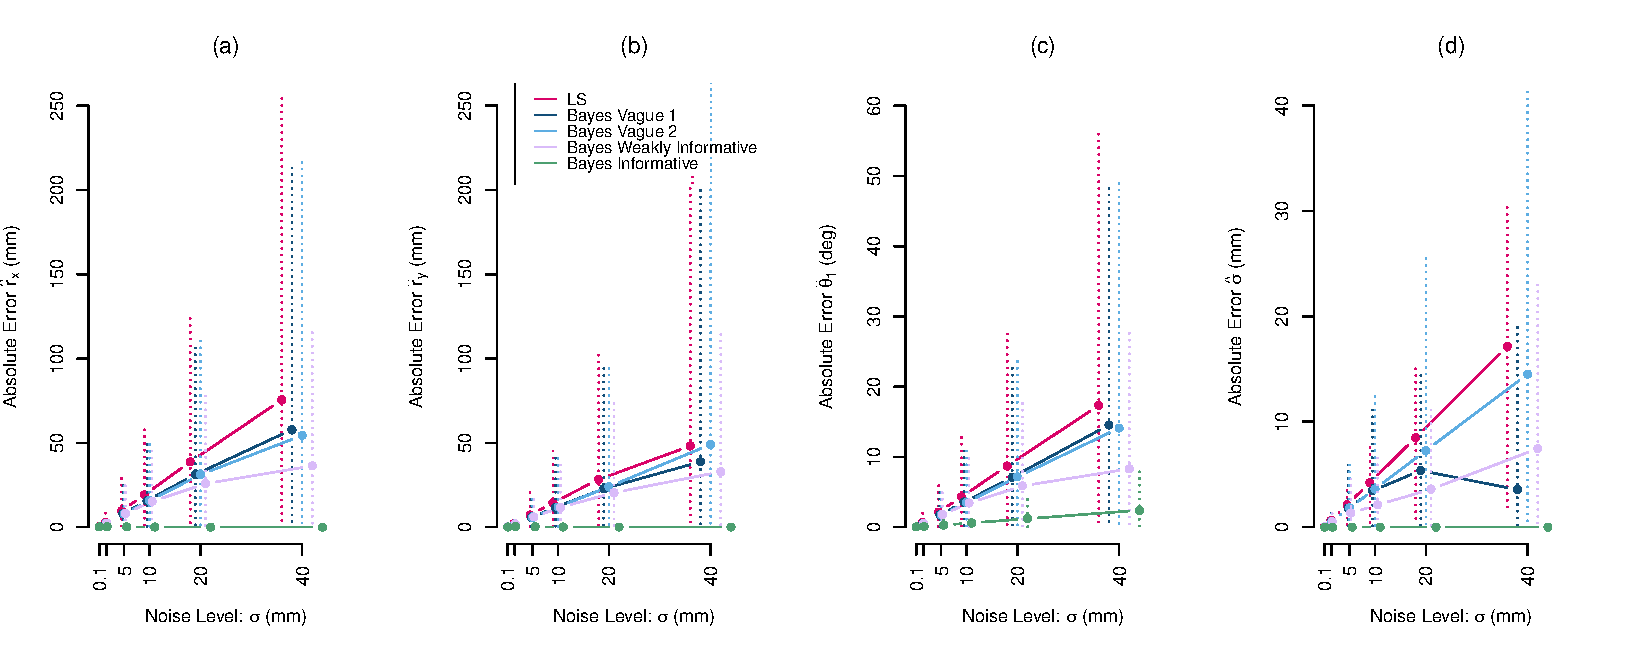
\includegraphics[width = \linewidth]{./Figures/LinePlot-Error-Legend}
	\caption{Median absolute error for each parameter at the 6 noise levels explored, (a)$r_x$, (b) $r_y$, (c) $\theta_1$ and (d) $\sigma$.  Dotted lines denote the 2.5th - 97.5th quantile range across the 1000 simulations. Note for visual clarity some horizontal jitter has been applied to separate results}
	\label{fig:LinePlotError}
\end{figure}
\begin{figure}.
	\centering
	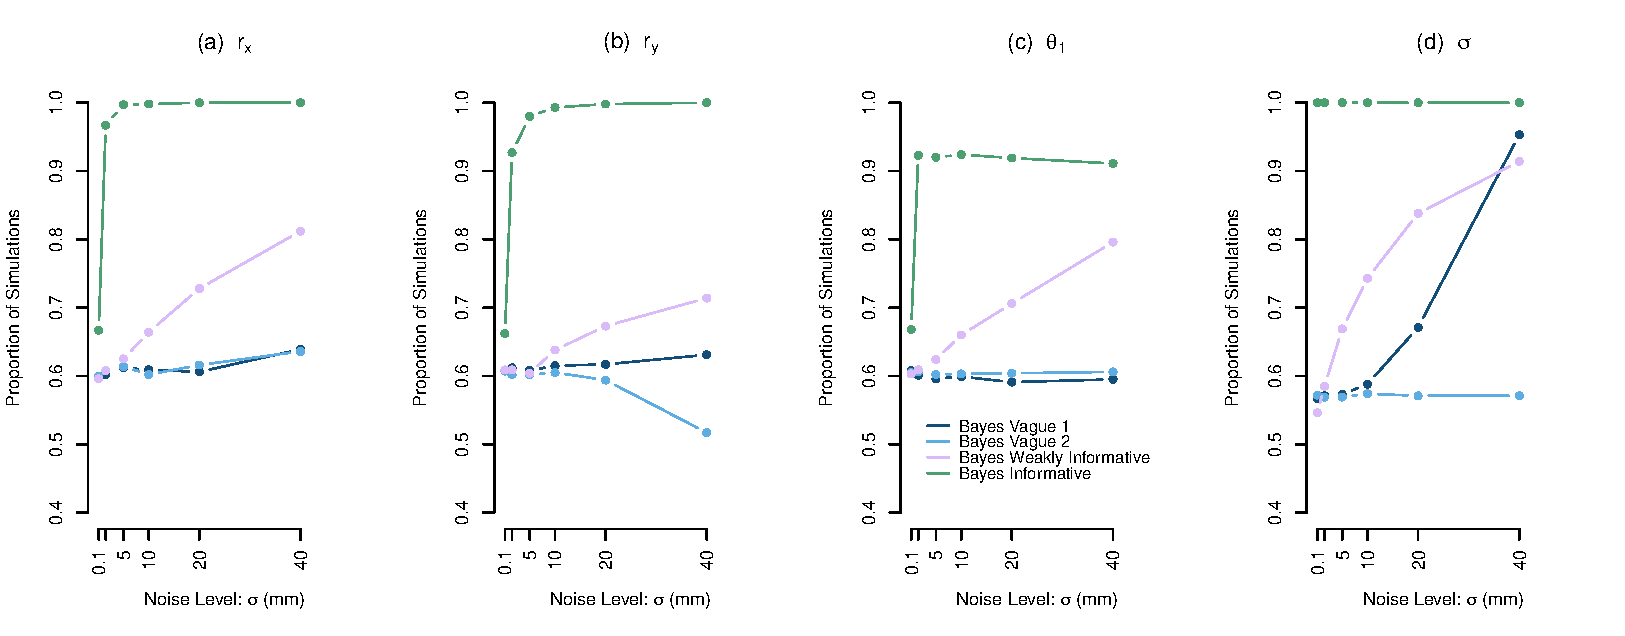
\includegraphics[width = \linewidth]{./Figures/LinePlot-Perf-legend}
	\caption{Proportion of 1000 simulations in which each Bayesian model had less absolute error than the corresponding LS estimator across each parameter: (a)$r_x$, (b) $r_y$, (c) $\theta_1$ and (d) $\sigma$. }
	\label{fig:LinePlotPerf}
\end{figure}

\section{Discussion}
In support of our hypotheses we observe that, with the exception of the model with a highly informative prior centred on the true values, estimator error increases with increasing noise (Figure \ref{fig:LinePlotError}).  The fact that a model with highly informative priors is robust to increasing measurement noise is not surprising and suggests that the prior distribution is overwhelming observed data. The fact that this prior is centred on the true values of the simulation and the prior overwhelms observed data results in this particular model being robust to any increases in noise within the system and as a result out performs the LS solution in 100\% of simulations when measurement noise is large ($>20\si{\milli\meter}$). However, it is important to note that such a prior is unable to be used in practice as, in practical application, the true values of a given kinematic pose are unknown (hence the need for a model to estimate these from noisy marker positions).

The absolute error for all other Bayesian models and the LS solution increases with increasing measurement noise.  This is a direct consequence of a reduction in the signal to noise ratio of the system.  However, the rate of increase in error is not constant for all models. Specifically while the rate of increase in absolute error for the model with the second set of vague priors (Vague 2) is not different from the LS solution within the range of tested measurement noise, the model with weakly informative priors begins to deviate at approximately 5\si{\milli\meter} and the model with the 1st set of vague priors (Vague 1) deviates at 40\si{\milli\meter} of measurement noise.  The deviation of these priors from the LS solution speaks to how informative these particular priors are.  At low noise levels both Vague 1 and the weakly informative prior are relatively non-informative and the data informed likelihood dominates the formulation of the posterior distribution.  However, as noise increases these priors become increasingly informative.  The constraints inherent to the use of uniform distributions over finite parameter intervals act as a filter to reduce the posterior probability of possible IK solutions which are not consistent with the prior distribution (in the case of vague 1, reducing this posterior probability to 0 for parameter values outside the range of marginal uniform prior distributions for each parameter). As a specific example, consider that a translation exceeding a magnitude of $1$\si{\meter} has zero posterior probability given the marginal $\text{Uniform}(\bm{-0.5}, \bm{0.5})$ prior distribution used for translation vector $\bm{r}$ in the `vague 1' model described in Figure \ref{fig:LinePlotError} and \ref{fig:LinePlotPerf}. When considering marker configurations observed under large magnitude noise these large magnitude translations have increased likelihood but are filtered by this `vague' prior.  

These observations are similar to what is described in \cite{serrien_bayesian_2020} in that the performance of Bayesian models with uniform vague priors qualitatively diverges from the LS solution at high levels of measurement noise ($>10\si{\milli\meter}$).  While the models explored in \cite{serrien_bayesian_2020} also include estimates of soft tissue artefact and are thus not directly comparable to those explored in this supplement, we suspect that `filtering' resulting from truncation of the sample space via the use of restricted uniform priors may partially explain these observations although further research and experimentation would be required to confirm this assertion.

This `filtering' is clearly observed in the right column of Figure \ref{fig:Error40scatter} which plots the Bayesian estimate against the LS estimator for each parameter and choice of Bayesian prior when 40\si{\milli\meter} of measurement noise is present within the system.  For vague 1 the upper limit of 50\si{\milli\meter} for measurement noise is clearly evident and acts to restrict posterior estimates below this value.  Similar, the physiological expectations described by the weakly informative prior have a similar effect in the 3rd plot of the right hand column.  
\begin{figure}.
	\centering
	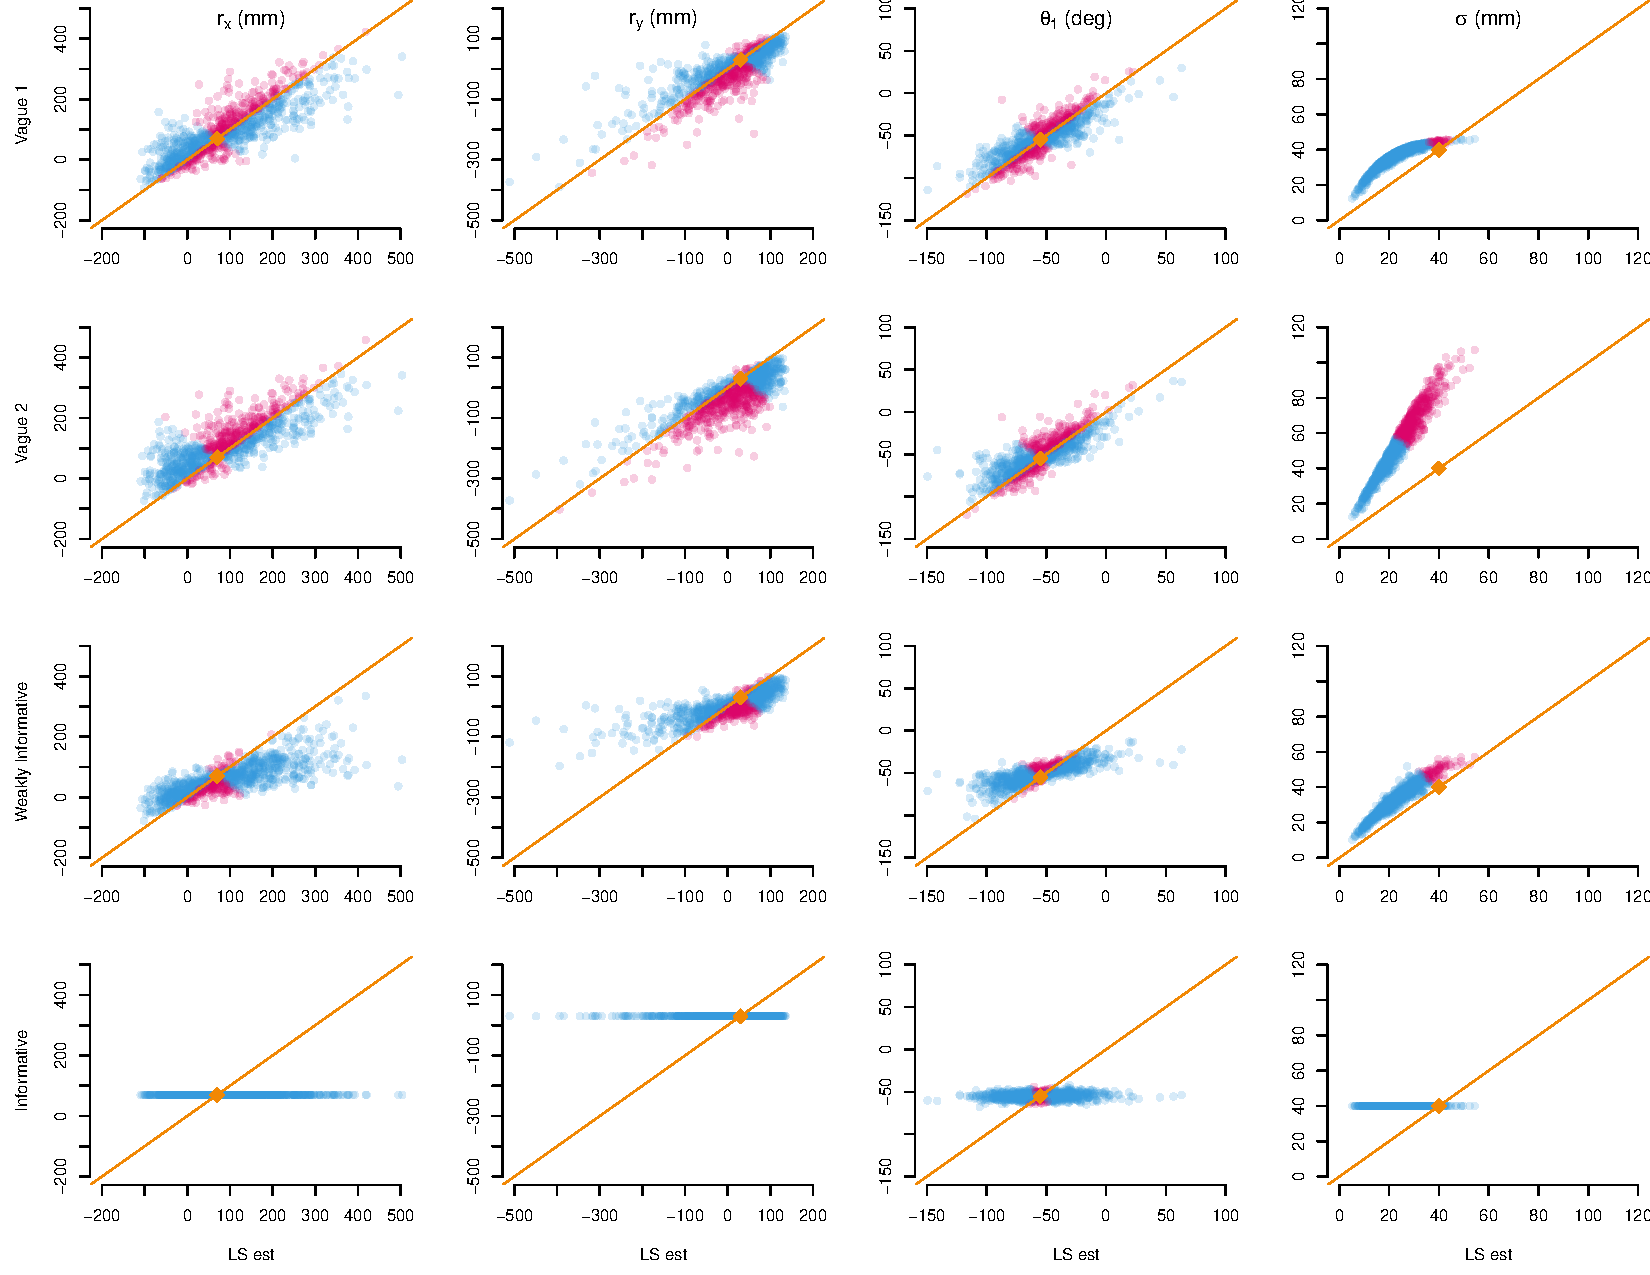
\includegraphics[width = \linewidth]{./Figures/Error40Scatter}
	\caption{The Bayesian estimate plotted against the LS estimate for each parameter (columns) and choice of prior (rows) when 40\si{\milli\meter} of measurement noise is present within the system.  The orange line depicts the 1-1 equivalence of the two estimates with the orange diamond describing the true value of the simulations.  Each of the simulations is identified in blue if the Bayes estimate has lower absolute error or pink if the LS estimator has lower absolute error.}
	\label{fig:Error40scatter}
\end{figure}

The difficulties in determining non-informative prior distributions which remain non-informative across differing scales of the parameter space are well known within the Bayesian community and historically have been a major criticism of the Bayesian approach to statistical inference \citep{gelman_objections_2008, efron_why_1986, gelman_prior_2006}.  A common example is when half uniform  or inverse-gamma($\epsilon, \epsilon$) priors are used for between group standard deviation parameters in hierarchical models \citep{gelman_prior_2006}.  Despite these priors being relatively non-informative at the scale of the standard deviation they exert surprising influence on the posterior distribution for between group variance \citep{gelman_prior_2006}.  Other common examples include `non-informative' priors placed over the natural scale of a parameter $\theta$ having surprising influence on the $\log(\theta)$. While there exists several `algorithmic' approaches to deriving non-informative priors \citep{kass_selection_1996} the modern approach is to specify weakly informative priors \citep{gelman_prior_2006}.  For this reason we encourage researchers looking to use Bayesian statistics for biomechanical analyses derive weakly informative priors based on results from previously published work.

\section{Conclusion}
The formulation of truly vague or un-informative priors is a challenging problem when using Bayesian inference for IK problems.  Priors which use uniform distributions over subsets of the possible sample space of pose parameters (e.g. Vague 1 and Vague 2 in this supplement) may seem to intuitively vague given they communicate equal probability across their support.  As we have observed in this supplement these priors can act as a filter when measurement noise increases reducing the posterior probability of poses outside the support of the prior to 0.  This results in these priors becoming increasingly informative and as a result reductions in estimator variance and improvements in accuracy when compared to traditional LS approaches are observed. This filtering property may help to explain the improvements in accuracy observed with increasing measurement noise observed by \cite{serrien_bayesian_2020} although further research should be conducted to validate this assertion.
\bibliography{References.bib}

\end{document}
